% !TEX root = ./../../_Thesis.tex

% section's Name and Label
\subsection{Comparison of Simulated Results with Ground Truth}
\label{sec:OpticalSimulation(Results)}

This section compares our simulated results with an optical ground truth, obtained by capturing images of the LogMAR charts shown in Figure~\ref{fig:etdrs_tables}.
%vision chart containing Sloan letters produced using Equation \ref{eq:lettersize} and placed at three feet from the camera. 
Whenever we reference to the dioptric power of additional lenses, our simulations account for the values described in Table~\ref{table:newDioptricPower}.  
%And even though the final arbiter of image quality is the human viewer, 
To objectively evaluate the quality of the simulated results, we use three objective metrics: the Structural Similarity Image Metric (SSIM)~\cite{Wang2004}, the Peak Signal-to-Noise Ratio (PSNR), and the Absolute Difference (AD) of the pixelwise differences between the captured and simulated images.
The SSIM metric measures image degradation perceived as change in structural information. 
%It produces a number between -1.0 (poor similarity) and 1.0 (high similarity). 
It is calculated for each pixel of a given image with respect to some reference image, based on its relationship to other pixels in an 11-by-11 neighborhood. PSNR is a popular metric in image processing for assessing the quality of image reconstruction and compression. It is often expressed using a decibel scale, and computed as  
%
\begin{equation}
	\centering
	\label{eq:PSNR}
	PSNR = 10\log_{10}\left (\frac{peakval^2}{MSE}\right ),
\end{equation}
where
\begin{equation}
	\centering
	\label{eq:MSE}
	MSE = \frac{1}{mn}\sum^{m-1}_{i=0}\sum^{n-1}_{j=0}(I_{ref}(i,j) - I(i,j))^2,
\end{equation}
and $I$ is an image being compared to a reference image $I_{ref}$, both with the same dimensions $m \times n$. 
$peakval$ is the maximum possible value for a pixel. For instance, for a grayscale image using 8-bits per pixel, $peakval=255$. 
   

%
The optical simulation described in this thesis was implemented using MATLAB Student Version (R2014a).
% environment has been chosen to implement the simulation technique described in this thesis. 
%
%As described in Section \ref{sec:Validation}, we've used additional lenses to induce low-order aberrations (\ie, myopia, hyperopia, and astigmatism) into a DSLR camera's optical system. This allow us to 
Figures~\ref{fig:comparison_myopic_wb} and \ref{fig:comparison_myopic_bw} compare images of a letter from the LogMAR charts with 
%Sloan letters against a 
white and black background, respectively, captured by the DSLR camera (top row) against the results of our simulations (second row). 
%of myopic views of the chart. 
The images in the top rows were captured by the camera with extra lenses, ranging from 0 to +4 diopters, in steps of 1 diopter. The second rows show the images produced using our simulation and considering the adjustments in dioptric power required to account for the 10mm spacing between the camera's main lens and the additional one (Table~\ref{table:newDioptricPower}). Our simulations were applied to the image captured by the camera without any extra lens (\ie, camera +0.00 D). The third and fourth rows of these figures show visual representations of the SSIM an AD metrics, respectively. 
%Also the comparison when using the SSIM metric (third row) or AD metric (bottom row).

% Myopic 		- Figures
% !TEX root = ./../../../_Thesis.tex

\begin{figure*}[!t]
	\centering
	
	\begin{tabular}{@{}r@{ } c@{ } c@{ } c@{ } c@{ } c }
	&
	\small{+0.00 D} &
	\small{+1.00 D} &
	\small{+2.00 D} &
	\small{+3.00 D} &
	\small{+4.00 D} & \\

	\begin{sideways} \parbox[b]{20mm} {Camera} \end{sideways} &
	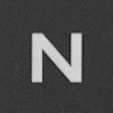
\includegraphics[width=0.185\textwidth]{__Images/05/BW_N(20-200)_+0D_to_+4D/bw_N_20-200_Camera+0,00D(lens).png} &
	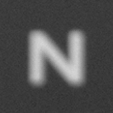
\includegraphics[width=0.185\textwidth]{__Images/05/BW_N(20-200)_+0D_to_+4D/bw_N_20-200_Camera+1,00D(lens).png} &
	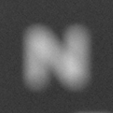
\includegraphics[width=0.185\textwidth]{__Images/05/BW_N(20-200)_+0D_to_+4D/bw_N_20-200_Camera+2,00D(lens).png} &
	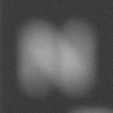
\includegraphics[width=0.185\textwidth]{__Images/05/BW_N(20-200)_+0D_to_+4D/bw_N_20-200_Camera+3,00D(lens).png} &
	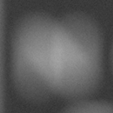
\includegraphics[width=0.185\textwidth]{__Images/05/BW_N(20-200)_+0D_to_+4D/bw_N_20-200_Camera+4,00D(lens).png} \\

	\begin{sideways} \parbox[b]{20mm} {Simulation} \end{sideways} &
	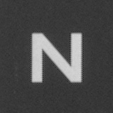
\includegraphics[width=0.185\textwidth]{__Images/05/BW_N(20-200)_+0D_to_+4D/bw_N_20-200_Camera+0,00D(simulated).png} &
	
\includegraphics[width=0.185\textwidth]{__Images/05/BW_N(20-200)_+0D_to_+4D/bw_N_20-200_Camera+1,00D(simulated).png} &
	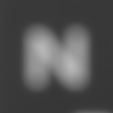
\includegraphics[width=0.185\textwidth]{__Images/05/BW_N(20-200)_+0D_to_+4D/bw_N_20-200_Camera+2,00D(simulated).png} &
	
\includegraphics[width=0.185\textwidth]{__Images/05/BW_N(20-200)_+0D_to_+4D/bw_N_20-200_Camera+3,00D(simulated).png} &
	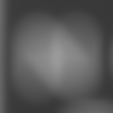
\includegraphics[width=0.185\textwidth]{__Images/05/BW_N(20-200)_+0D_to_+4D/bw_N_20-200_Camera+4,00D(simulated).png} \\

	\begin{sideways} \parbox[b]{20mm} {Local~SSIM} \end{sideways} &
	
\includegraphics[width=0.185\textwidth]{__Images/05/BW_N(20-200)_+0D_to_+4D/bw_N_20-200_Camera+0,00D(comparison).png} &
	
\includegraphics[width=0.185\textwidth]{__Images/05/BW_N(20-200)_+0D_to_+4D/bw_N_20-200_Camera+1,00D(comparison).png} &
	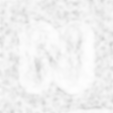
\includegraphics[width=0.185\textwidth]{__Images/05/BW_N(20-200)_+0D_to_+4D/bw_N_20-200_Camera+2,00D(comparison).png} &
	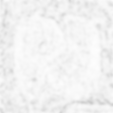
\includegraphics[width=0.185\textwidth]{__Images/05/BW_N(20-200)_+0D_to_+4D/bw_N_20-200_Camera+3,00D(comparison).png} &
	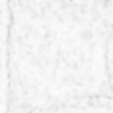
\includegraphics[width=0.185\textwidth]{__Images/05/BW_N(20-200)_+0D_to_+4D/bw_N_20-200_Camera+4,00D(comparison).png} \\
	
	\begin{sideways} \parbox[b]{20mm} {Difference} \end{sideways} &
	
\includegraphics[width=0.185\textwidth]{__Images/05/BW_N(20-200)_+0D_to_+4D/bw_N_20-200_Camera+0,00D(diff).png} &
	
\includegraphics[width=0.185\textwidth]{__Images/05/BW_N(20-200)_+0D_to_+4D/bw_N_20-200_Camera+1,00D(diff).png} &
	
\includegraphics[width=0.185\textwidth]{__Images/05/BW_N(20-200)_+0D_to_+4D/bw_N_20-200_Camera+2,00D(diff).png} &
	
\includegraphics[width=0.185\textwidth]{__Images/05/BW_N(20-200)_+0D_to_+4D/bw_N_20-200_Camera+3,00D(diff).png} &
	
\includegraphics[width=0.185\textwidth]{__Images/05/BW_N(20-200)_+0D_to_+4D/bw_N_20-200_Camera+4,00D(diff).png} \\
 
	\end{tabular}
	
	\caption[Comparisons of our simulated results against ground truth obtained with a myopic camera]{Comparisons of our simulated results against ground truth obtained with a myopic camera. These images correspond to a Snellen ratio of 20/200.   (top row) Images captured using the DSLR camera with extra lenses varying from 0.0 to 4.0 diopters. (second row) Our simulated results. (third row) SSIM metric results. (fourth row) AD metric. } %BW, N, 20/200, +0 +1 +2 +3 +4
	\label{fig:comparison_myopic_bw}
\end{figure*}	% fig:comparison_myopic_wb
% !TEX root = ./../../../_Thesis.tex

\begin{figure*}[!t]
	\centering
	
	\begin{tabular}{@{}r@{ } c@{ } c@{ } c@{ } c@{ } c }
	&
	\small{+0.00 D} &
	\small{+1.00 D} &
	\small{+2.00 D} &
	\small{+3.00 D} &
	\small{+4.00 D} & \\

	\begin{sideways} \parbox[b]{20mm} {Camera} \end{sideways} &
	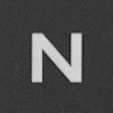
\includegraphics[width=0.185\textwidth]{__Images/05/BW_N(20-200)_+0D_to_+4D/bw_N_20-200_Camera+0,00D(lens).png} &
	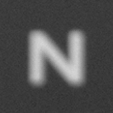
\includegraphics[width=0.185\textwidth]{__Images/05/BW_N(20-200)_+0D_to_+4D/bw_N_20-200_Camera+1,00D(lens).png} &
	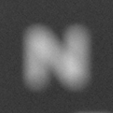
\includegraphics[width=0.185\textwidth]{__Images/05/BW_N(20-200)_+0D_to_+4D/bw_N_20-200_Camera+2,00D(lens).png} &
	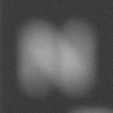
\includegraphics[width=0.185\textwidth]{__Images/05/BW_N(20-200)_+0D_to_+4D/bw_N_20-200_Camera+3,00D(lens).png} &
	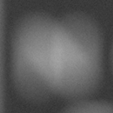
\includegraphics[width=0.185\textwidth]{__Images/05/BW_N(20-200)_+0D_to_+4D/bw_N_20-200_Camera+4,00D(lens).png} \\

	\begin{sideways} \parbox[b]{20mm} {Simulation} \end{sideways} &
	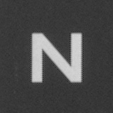
\includegraphics[width=0.185\textwidth]{__Images/05/BW_N(20-200)_+0D_to_+4D/bw_N_20-200_Camera+0,00D(simulated).png} &
	
\includegraphics[width=0.185\textwidth]{__Images/05/BW_N(20-200)_+0D_to_+4D/bw_N_20-200_Camera+1,00D(simulated).png} &
	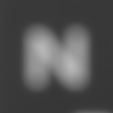
\includegraphics[width=0.185\textwidth]{__Images/05/BW_N(20-200)_+0D_to_+4D/bw_N_20-200_Camera+2,00D(simulated).png} &
	
\includegraphics[width=0.185\textwidth]{__Images/05/BW_N(20-200)_+0D_to_+4D/bw_N_20-200_Camera+3,00D(simulated).png} &
	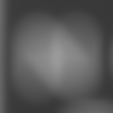
\includegraphics[width=0.185\textwidth]{__Images/05/BW_N(20-200)_+0D_to_+4D/bw_N_20-200_Camera+4,00D(simulated).png} \\

	\begin{sideways} \parbox[b]{20mm} {Local~SSIM} \end{sideways} &
	
\includegraphics[width=0.185\textwidth]{__Images/05/BW_N(20-200)_+0D_to_+4D/bw_N_20-200_Camera+0,00D(comparison).png} &
	
\includegraphics[width=0.185\textwidth]{__Images/05/BW_N(20-200)_+0D_to_+4D/bw_N_20-200_Camera+1,00D(comparison).png} &
	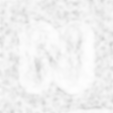
\includegraphics[width=0.185\textwidth]{__Images/05/BW_N(20-200)_+0D_to_+4D/bw_N_20-200_Camera+2,00D(comparison).png} &
	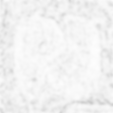
\includegraphics[width=0.185\textwidth]{__Images/05/BW_N(20-200)_+0D_to_+4D/bw_N_20-200_Camera+3,00D(comparison).png} &
	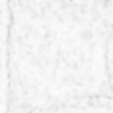
\includegraphics[width=0.185\textwidth]{__Images/05/BW_N(20-200)_+0D_to_+4D/bw_N_20-200_Camera+4,00D(comparison).png} \\
	
	\begin{sideways} \parbox[b]{20mm} {Difference} \end{sideways} &
	
\includegraphics[width=0.185\textwidth]{__Images/05/BW_N(20-200)_+0D_to_+4D/bw_N_20-200_Camera+0,00D(diff).png} &
	
\includegraphics[width=0.185\textwidth]{__Images/05/BW_N(20-200)_+0D_to_+4D/bw_N_20-200_Camera+1,00D(diff).png} &
	
\includegraphics[width=0.185\textwidth]{__Images/05/BW_N(20-200)_+0D_to_+4D/bw_N_20-200_Camera+2,00D(diff).png} &
	
\includegraphics[width=0.185\textwidth]{__Images/05/BW_N(20-200)_+0D_to_+4D/bw_N_20-200_Camera+3,00D(diff).png} &
	
\includegraphics[width=0.185\textwidth]{__Images/05/BW_N(20-200)_+0D_to_+4D/bw_N_20-200_Camera+4,00D(diff).png} \\
 
	\end{tabular}
	
	\caption[Comparisons of our simulated results against ground truth obtained with a myopic camera]{Comparisons of our simulated results against ground truth obtained with a myopic camera. These images correspond to a Snellen ratio of 20/200.   (top row) Images captured using the DSLR camera with extra lenses varying from 0.0 to 4.0 diopters. (second row) Our simulated results. (third row) SSIM metric results. (fourth row) AD metric. } %BW, N, 20/200, +0 +1 +2 +3 +4
	\label{fig:comparison_myopic_bw}
\end{figure*}	% fig:comparison_myopic_bw

%\startsquarepar
Tables~\ref{table:metrics_myopic_wb} and \ref{table:metrics_myopic_bw} show the numerical results of the SSIM and PSNR metrics for the results presented in Figures~\ref{fig:comparison_myopic_wb} and \ref{fig:comparison_myopic_bw}, respectively. Each row represents the value of a specific metric (\ie, SSIM or PSNR) when comparing an image captured by the DSLR camera with the one obtained using our simulation.  
The values of the SSIM metric range from 0.0 (poor similarity) to 1.0 (high similarity). In these tables, one can see that all values are very close to 1.0, indicating that our simulations indeed produces results that are structurally very  similar the ground truth. The PSNR values also indicate that our simulations also produce results very similar to the ground truth. Note that PSNR values of 34.0 decibels and above indicate that two images are essentially indistinguishable from each other.  

%It is possible to visualize the results of this metric as an image, which represents the local (\ie, pixel-by-pixel) SSIM index. Such images are illustrated in Figures~\ref{fig:comparison_myopic_wb}(third row) and \ref{fig:comparison_myopic_bw}(third row). We've obtained the PSNR by calculating the mean squared error (MSE) and then dividing the maximum signal value that exists in our optical ground truth image by the MSE. This metric is given in decibel and relies strictly on numeric comparison between images. When two images are identical, the PSNR tends to infinity. Excellent values range from 30 to 50 dB, where higher is better.
%\stopsquarepar

% Myopic 		- Tables
% !TEX root = ./../../../_Thesis.tex

\begin{table}[!b]
	\centering
	\label{table:metrics_hyperopic_wb}
	\caption[SSIM and PSNR table of hyperopic perception (Figure~\ref{fig:comparison_hyperopic_wb})]{SSIM and PSNR table of hyperopic perception (Figure~\ref{fig:comparison_hyperopic_wb})}
	
	\begin{tabular}{cccccc}
	{\bf }                          & {\bf -0.00 D} & {\bf -1.00 D} & {\bf -2.00 D} & {\bf -3.00 D} & {\bf -4.00 D} \\ \hline
	\multicolumn{1}{c|}{{\bf SSIM}} & 0.9869  		& 0.9192  		& 0.9149  		& 0.9119  		& 0.9130  		\\
	\multicolumn{1}{c|}{{\bf PSNR}} & 34.7778 		& 34.3781 		& 32.8601 		& 32.6680 		& 29.5003
	\end{tabular}
\end{table}	% table:metrics_myopic_wb
% !TEX root = ./../../../_Thesis.tex

\begin{table}[!b]
	\centering
	\label{table:metrics_hyperopic_wb}
	\caption[SSIM and PSNR table of hyperopic perception (Figure~\ref{fig:comparison_hyperopic_wb})]{SSIM and PSNR table of hyperopic perception (Figure~\ref{fig:comparison_hyperopic_wb})}
	
	\begin{tabular}{cccccc}
	{\bf }                          & {\bf -0.00 D} & {\bf -1.00 D} & {\bf -2.00 D} & {\bf -3.00 D} & {\bf -4.00 D} \\ \hline
	\multicolumn{1}{c|}{{\bf SSIM}} & 0.9869  		& 0.9192  		& 0.9149  		& 0.9119  		& 0.9130  		\\
	\multicolumn{1}{c|}{{\bf PSNR}} & 34.7778 		& 34.3781 		& 32.8601 		& 32.6680 		& 29.5003
	\end{tabular}
\end{table}	% table:metrics_myopic_bw

%\noindent

Figures~\ref{fig:comparison_hyperopic_wb} and \ref{fig:comparison_hyperopic_bw} provide similar comparisons for hyperopic vision. The results in the top row were captured with a DSLR camera and extra lenses ranging from 0 to -4 diopters, in steps of -1 diopter. The second rows show our simulated results. Likewise, the third row presents the visualization of the pixel-by-pixel SSIM index when comparing the captured and simulated hyperopic results, and the bottom one presents the absolute difference of images. Tables~\ref{table:metrics_hyperopic_wb} and \ref{table:metrics_hyperopic_bw} provide the SSIM and PSNR values comparing the simulated images to the ground truth, attesting the quality of our results. 

% Hyperopic 	- Figures and Tables
% !TEX root = ./../../../_Thesis.tex

\begin{figure*}[!t]
	\centering
	
	\begin{tabular}{@{}r@{ } c@{ } c@{ } c@{ } c@{ } c }
	&
	\small{+0.00 D} &
	\small{+1.00 D} &
	\small{+2.00 D} &
	\small{+3.00 D} &
	\small{+4.00 D} & \\

	\begin{sideways} \parbox[b]{20mm} {Camera} \end{sideways} &
	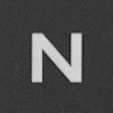
\includegraphics[width=0.185\textwidth]{__Images/05/BW_N(20-200)_+0D_to_+4D/bw_N_20-200_Camera+0,00D(lens).png} &
	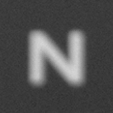
\includegraphics[width=0.185\textwidth]{__Images/05/BW_N(20-200)_+0D_to_+4D/bw_N_20-200_Camera+1,00D(lens).png} &
	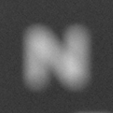
\includegraphics[width=0.185\textwidth]{__Images/05/BW_N(20-200)_+0D_to_+4D/bw_N_20-200_Camera+2,00D(lens).png} &
	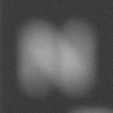
\includegraphics[width=0.185\textwidth]{__Images/05/BW_N(20-200)_+0D_to_+4D/bw_N_20-200_Camera+3,00D(lens).png} &
	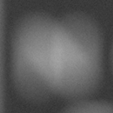
\includegraphics[width=0.185\textwidth]{__Images/05/BW_N(20-200)_+0D_to_+4D/bw_N_20-200_Camera+4,00D(lens).png} \\

	\begin{sideways} \parbox[b]{20mm} {Simulation} \end{sideways} &
	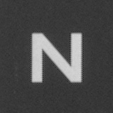
\includegraphics[width=0.185\textwidth]{__Images/05/BW_N(20-200)_+0D_to_+4D/bw_N_20-200_Camera+0,00D(simulated).png} &
	
\includegraphics[width=0.185\textwidth]{__Images/05/BW_N(20-200)_+0D_to_+4D/bw_N_20-200_Camera+1,00D(simulated).png} &
	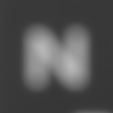
\includegraphics[width=0.185\textwidth]{__Images/05/BW_N(20-200)_+0D_to_+4D/bw_N_20-200_Camera+2,00D(simulated).png} &
	
\includegraphics[width=0.185\textwidth]{__Images/05/BW_N(20-200)_+0D_to_+4D/bw_N_20-200_Camera+3,00D(simulated).png} &
	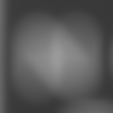
\includegraphics[width=0.185\textwidth]{__Images/05/BW_N(20-200)_+0D_to_+4D/bw_N_20-200_Camera+4,00D(simulated).png} \\

	\begin{sideways} \parbox[b]{20mm} {Local~SSIM} \end{sideways} &
	\includegraphics[width=0.185\textwidth]{__Images/05/BW_N(20-200)_+0D_to_+4D/bw_N_20-200_Camera+0,00D(comparison).png} &
	\includegraphics[width=0.185\textwidth]{__Images/05/BW_N(20-200)_+0D_to_+4D/bw_N_20-200_Camera+1,00D(comparison).png} &
	\includegraphics[width=0.185\textwidth]{__Images/05/BW_N(20-200)_+0D_to_+4D/bw_N_20-200_Camera+2,00D(comparison).png} &
	\includegraphics[width=0.185\textwidth]{__Images/05/BW_N(20-200)_+0D_to_+4D/bw_N_20-200_Camera+3,00D(comparison).png} &
	\includegraphics[width=0.185\textwidth]{__Images/05/BW_N(20-200)_+0D_to_+4D/bw_N_20-200_Camera+4,00D(comparison).png} \\
	
	\begin{sideways} \parbox[b]{20mm} {Difference} \end{sideways} &
	\includegraphics[width=0.185\textwidth]{__Images/05/BW_N(20-200)_+0D_to_+4D/bw_N_20-200_Camera+0,00D(diff).png} &
	\includegraphics[width=0.185\textwidth]{__Images/05/BW_N(20-200)_+0D_to_+4D/bw_N_20-200_Camera+1,00D(diff).png} &
	\includegraphics[width=0.185\textwidth]{__Images/05/BW_N(20-200)_+0D_to_+4D/bw_N_20-200_Camera+2,00D(diff).png} &
	\includegraphics[width=0.185\textwidth]{__Images/05/BW_N(20-200)_+0D_to_+4D/bw_N_20-200_Camera+3,00D(diff).png} &
	\includegraphics[width=0.185\textwidth]{__Images/05/BW_N(20-200)_+0D_to_+4D/bw_N_20-200_Camera+4,00D(diff).png} \\
 
	\end{tabular}
	
	\caption[Comparisons of our simulated results against ground truth obtained with a myopic camera]{Comparisons of our simulated results against ground truth obtained with a myopic camera. These images correspond to a Snellen ratio of 20/200.   (top row) Images captured using the DSLR camera with extra lenses varying from 0.0 to 4.0 diopters. (second row) Our simulated results. (third row) SSIM metric results. (fourth row) AD metric. } %BW, N, 20/200, +0 +1 +2 +3 +4
	\label{fig:comparison_myopic_bw}
\end{figure*}	% fig:comparison_hyperopic_wb
% !TEX root = ./../../../_Thesis.tex

\begin{table}[!b]
	\centering
	\label{table:metrics_hyperopic_wb}
	\caption[SSIM and PSNR table of hyperopic perception (Figure~\ref{fig:comparison_hyperopic_wb})]{SSIM and PSNR table of hyperopic perception (Figure~\ref{fig:comparison_hyperopic_wb})}
	
	\begin{tabular}{cccccc}
	{\bf }                          & {\bf -0.00 D} & {\bf -1.00 D} & {\bf -2.00 D} & {\bf -3.00 D} & {\bf -4.00 D} \\ \hline
	\multicolumn{1}{c|}{{\bf SSIM}} & 0.9869  		& 0.9192  		& 0.9149  		& 0.9119  		& 0.9130  		\\
	\multicolumn{1}{c|}{{\bf PSNR}} & 34.7778 		& 34.3781 		& 32.8601 		& 32.6680 		& 29.5003
	\end{tabular}
\end{table}	% table:metrics_hyperopic_wb
% !TEX root = ./../../../_Thesis.tex

\begin{table}[!b]
	\centering
	\label{table:metrics_hyperopic_wb}
	\caption[SSIM and PSNR table of hyperopic perception (Figure~\ref{fig:comparison_hyperopic_wb})]{SSIM and PSNR table of hyperopic perception (Figure~\ref{fig:comparison_hyperopic_wb})}
	
	\begin{tabular}{cccccc}
	{\bf }                          & {\bf -0.00 D} & {\bf -1.00 D} & {\bf -2.00 D} & {\bf -3.00 D} & {\bf -4.00 D} \\ \hline
	\multicolumn{1}{c|}{{\bf SSIM}} & 0.9869  		& 0.9192  		& 0.9149  		& 0.9119  		& 0.9130  		\\
	\multicolumn{1}{c|}{{\bf PSNR}} & 34.7778 		& 34.3781 		& 32.8601 		& 32.6680 		& 29.5003
	\end{tabular}
\end{table}	% table:metrics_hyperopic_bw
% !TEX root = ./../../../_Thesis.tex

\begin{figure*}[!t]
	\centering
	
	\begin{tabular}{@{}r@{ } c@{ } c@{ } c@{ } c@{ } c }
	&
	\small{+0.00 D} &
	\small{+1.00 D} &
	\small{+2.00 D} &
	\small{+3.00 D} &
	\small{+4.00 D} & \\

	\begin{sideways} \parbox[b]{20mm} {Camera} \end{sideways} &
	\includegraphics[width=0.185\textwidth]{__Images/05/BW_N(20-200)_+0D_to_+4D/bw_N_20-200_Camera+0,00D(lens).png} &
	\includegraphics[width=0.185\textwidth]{__Images/05/BW_N(20-200)_+0D_to_+4D/bw_N_20-200_Camera+1,00D(lens).png} &
	\includegraphics[width=0.185\textwidth]{__Images/05/BW_N(20-200)_+0D_to_+4D/bw_N_20-200_Camera+2,00D(lens).png} &
	\includegraphics[width=0.185\textwidth]{__Images/05/BW_N(20-200)_+0D_to_+4D/bw_N_20-200_Camera+3,00D(lens).png} &
	\includegraphics[width=0.185\textwidth]{__Images/05/BW_N(20-200)_+0D_to_+4D/bw_N_20-200_Camera+4,00D(lens).png} \\

	\begin{sideways} \parbox[b]{20mm} {Simulation} \end{sideways} &
	\includegraphics[width=0.185\textwidth]{__Images/05/BW_N(20-200)_+0D_to_+4D/bw_N_20-200_Camera+0,00D(simulated).png} &
	\includegraphics[width=0.185\textwidth]{__Images/05/BW_N(20-200)_+0D_to_+4D/bw_N_20-200_Camera+1,00D(simulated).png} &
	\includegraphics[width=0.185\textwidth]{__Images/05/BW_N(20-200)_+0D_to_+4D/bw_N_20-200_Camera+2,00D(simulated).png} &
	\includegraphics[width=0.185\textwidth]{__Images/05/BW_N(20-200)_+0D_to_+4D/bw_N_20-200_Camera+3,00D(simulated).png} &
	\includegraphics[width=0.185\textwidth]{__Images/05/BW_N(20-200)_+0D_to_+4D/bw_N_20-200_Camera+4,00D(simulated).png} \\

	\begin{sideways} \parbox[b]{20mm} {Local~SSIM} \end{sideways} &
	\includegraphics[width=0.185\textwidth]{__Images/05/BW_N(20-200)_+0D_to_+4D/bw_N_20-200_Camera+0,00D(comparison).png} &
	\includegraphics[width=0.185\textwidth]{__Images/05/BW_N(20-200)_+0D_to_+4D/bw_N_20-200_Camera+1,00D(comparison).png} &
	\includegraphics[width=0.185\textwidth]{__Images/05/BW_N(20-200)_+0D_to_+4D/bw_N_20-200_Camera+2,00D(comparison).png} &
	\includegraphics[width=0.185\textwidth]{__Images/05/BW_N(20-200)_+0D_to_+4D/bw_N_20-200_Camera+3,00D(comparison).png} &
	\includegraphics[width=0.185\textwidth]{__Images/05/BW_N(20-200)_+0D_to_+4D/bw_N_20-200_Camera+4,00D(comparison).png} \\
	
	\begin{sideways} \parbox[b]{20mm} {Difference} \end{sideways} &
	\includegraphics[width=0.185\textwidth]{__Images/05/BW_N(20-200)_+0D_to_+4D/bw_N_20-200_Camera+0,00D(diff).png} &
	\includegraphics[width=0.185\textwidth]{__Images/05/BW_N(20-200)_+0D_to_+4D/bw_N_20-200_Camera+1,00D(diff).png} &
	\includegraphics[width=0.185\textwidth]{__Images/05/BW_N(20-200)_+0D_to_+4D/bw_N_20-200_Camera+2,00D(diff).png} &
	\includegraphics[width=0.185\textwidth]{__Images/05/BW_N(20-200)_+0D_to_+4D/bw_N_20-200_Camera+3,00D(diff).png} &
	\includegraphics[width=0.185\textwidth]{__Images/05/BW_N(20-200)_+0D_to_+4D/bw_N_20-200_Camera+4,00D(diff).png} \\
 
	\end{tabular}
	
	\caption[Comparisons of our simulated results against ground truth obtained with a myopic camera]{Comparisons of our simulated results against ground truth obtained with a myopic camera. These images correspond to a Snellen ratio of 20/200.   (top row) Images captured using the DSLR camera with extra lenses varying from 0.0 to 4.0 diopters. (second row) Our simulated results. (third row) SSIM metric results. (fourth row) AD metric. } %BW, N, 20/200, +0 +1 +2 +3 +4
	\label{fig:comparison_myopic_bw}
\end{figure*}	% fig:comparison_hyperopic_bw

Besides simulating the effects of defocus (\ie, myopia and hyperopia), we have also compared the results of our simulation for astigmatic vision.
%We've also explored simulations of more effects rather than defocus. 
This is illustrated in Figures~\ref{fig:comparison_astig-2@90_wb} and \ref{fig:comparison_astig-2@180_wb}.
% shows the simulation of an astigmatic perception. % cylindrical lens with -2 diopters at the vertical meridian
The Sloan letters in Figure~\ref{fig:comparison_astig-2@90_wb} were captured by the DSLR camera with an additional cylindrical lens with -2.0 diopters, rotated in order to simulate astigmatism in the horizontal meridian ($\phi = 90^{\circ}$). Similarly, Figure~\ref{fig:comparison_astig-2@180_wb} shows the real and simulated astigmatism in the vertical meridian ($\phi = 180^{\circ}$). 
Figures~\ref{fig:comparison_astig+2@90_bw} and \ref{fig:comparison_astig+2@180_bw} show the captured and simulated results for a cylindrical lens with +2.0 diopters. 
Tables~\ref{table:metrics_astig-2} and \ref{table:metrics_astig+2} show the results of the SSIM and PSNR metrics for these astigmatic results. Again, the SSIM indices are close 1.0 and the PSNR is close to or above 34.00 decibels.
%Both astigmatic simulations outcomes were evaluated using the SSIM and PSNR metrics, and the resultant values when comparing the simulated images to the reference ones are shown in .

Note that for the astigmatic results, part of the differences visible in 
the astigmatic local SSIM index visualizations (Figures~\ref{fig:comparison_astig-2@90_wb}, \ref{fig:comparison_astig-2@180_wb}, \ref{fig:comparison_astig+2@90_bw} and \ref{fig:comparison_astig+2@180_bw}) is due to the difficulty of a precise manual alignment of the astigmatic axes to the ones used in our simulations. Any deviation from the simulated angles affects the results of the quality metric.

% !TEX root = ./../../../_Thesis.tex

\begin{figure*}[!t]
	\centering
	
	\begin{tabular}{@{}r@{ } c@{ } c@{ } c@{ } c@{ } c }
	&
	\small{+0.00 D} &
	\small{+1.00 D} &
	\small{+2.00 D} &
	\small{+3.00 D} &
	\small{+4.00 D} & \\

	\begin{sideways} \parbox[b]{20mm} {Camera} \end{sideways} &
	\includegraphics[width=0.185\textwidth]{__Images/05/BW_N(20-200)_+0D_to_+4D/bw_N_20-200_Camera+0,00D(lens).png} &
	\includegraphics[width=0.185\textwidth]{__Images/05/BW_N(20-200)_+0D_to_+4D/bw_N_20-200_Camera+1,00D(lens).png} &
	\includegraphics[width=0.185\textwidth]{__Images/05/BW_N(20-200)_+0D_to_+4D/bw_N_20-200_Camera+2,00D(lens).png} &
	\includegraphics[width=0.185\textwidth]{__Images/05/BW_N(20-200)_+0D_to_+4D/bw_N_20-200_Camera+3,00D(lens).png} &
	\includegraphics[width=0.185\textwidth]{__Images/05/BW_N(20-200)_+0D_to_+4D/bw_N_20-200_Camera+4,00D(lens).png} \\

	\begin{sideways} \parbox[b]{20mm} {Simulation} \end{sideways} &
	\includegraphics[width=0.185\textwidth]{__Images/05/BW_N(20-200)_+0D_to_+4D/bw_N_20-200_Camera+0,00D(simulated).png} &
	\includegraphics[width=0.185\textwidth]{__Images/05/BW_N(20-200)_+0D_to_+4D/bw_N_20-200_Camera+1,00D(simulated).png} &
	\includegraphics[width=0.185\textwidth]{__Images/05/BW_N(20-200)_+0D_to_+4D/bw_N_20-200_Camera+2,00D(simulated).png} &
	\includegraphics[width=0.185\textwidth]{__Images/05/BW_N(20-200)_+0D_to_+4D/bw_N_20-200_Camera+3,00D(simulated).png} &
	\includegraphics[width=0.185\textwidth]{__Images/05/BW_N(20-200)_+0D_to_+4D/bw_N_20-200_Camera+4,00D(simulated).png} \\

	\begin{sideways} \parbox[b]{20mm} {Local~SSIM} \end{sideways} &
	\includegraphics[width=0.185\textwidth]{__Images/05/BW_N(20-200)_+0D_to_+4D/bw_N_20-200_Camera+0,00D(comparison).png} &
	\includegraphics[width=0.185\textwidth]{__Images/05/BW_N(20-200)_+0D_to_+4D/bw_N_20-200_Camera+1,00D(comparison).png} &
	\includegraphics[width=0.185\textwidth]{__Images/05/BW_N(20-200)_+0D_to_+4D/bw_N_20-200_Camera+2,00D(comparison).png} &
	\includegraphics[width=0.185\textwidth]{__Images/05/BW_N(20-200)_+0D_to_+4D/bw_N_20-200_Camera+3,00D(comparison).png} &
	\includegraphics[width=0.185\textwidth]{__Images/05/BW_N(20-200)_+0D_to_+4D/bw_N_20-200_Camera+4,00D(comparison).png} \\
	
	\begin{sideways} \parbox[b]{20mm} {Difference} \end{sideways} &
	\includegraphics[width=0.185\textwidth]{__Images/05/BW_N(20-200)_+0D_to_+4D/bw_N_20-200_Camera+0,00D(diff).png} &
	\includegraphics[width=0.185\textwidth]{__Images/05/BW_N(20-200)_+0D_to_+4D/bw_N_20-200_Camera+1,00D(diff).png} &
	\includegraphics[width=0.185\textwidth]{__Images/05/BW_N(20-200)_+0D_to_+4D/bw_N_20-200_Camera+2,00D(diff).png} &
	\includegraphics[width=0.185\textwidth]{__Images/05/BW_N(20-200)_+0D_to_+4D/bw_N_20-200_Camera+3,00D(diff).png} &
	\includegraphics[width=0.185\textwidth]{__Images/05/BW_N(20-200)_+0D_to_+4D/bw_N_20-200_Camera+4,00D(diff).png} \\
 
	\end{tabular}
	
	\caption[Comparisons of our simulated results against ground truth obtained with a myopic camera]{Comparisons of our simulated results against ground truth obtained with a myopic camera. These images correspond to a Snellen ratio of 20/200.   (top row) Images captured using the DSLR camera with extra lenses varying from 0.0 to 4.0 diopters. (second row) Our simulated results. (third row) SSIM metric results. (fourth row) AD metric. } %BW, N, 20/200, +0 +1 +2 +3 +4
	\label{fig:comparison_myopic_bw}
\end{figure*}			% fig:comparison_astig-2@90_wb
% !TEX root = ./../../../_Thesis.tex

\begin{figure*}[!t]
	\centering
	
	\begin{tabular}{@{}r@{ } c@{ } c@{ } c@{ } c@{ } c }
	&
	\small{+0.00 D} &
	\small{+1.00 D} &
	\small{+2.00 D} &
	\small{+3.00 D} &
	\small{+4.00 D} & \\

	\begin{sideways} \parbox[b]{20mm} {Camera} \end{sideways} &
	\includegraphics[width=0.185\textwidth]{__Images/05/BW_N(20-200)_+0D_to_+4D/bw_N_20-200_Camera+0,00D(lens).png} &
	\includegraphics[width=0.185\textwidth]{__Images/05/BW_N(20-200)_+0D_to_+4D/bw_N_20-200_Camera+1,00D(lens).png} &
	\includegraphics[width=0.185\textwidth]{__Images/05/BW_N(20-200)_+0D_to_+4D/bw_N_20-200_Camera+2,00D(lens).png} &
	\includegraphics[width=0.185\textwidth]{__Images/05/BW_N(20-200)_+0D_to_+4D/bw_N_20-200_Camera+3,00D(lens).png} &
	\includegraphics[width=0.185\textwidth]{__Images/05/BW_N(20-200)_+0D_to_+4D/bw_N_20-200_Camera+4,00D(lens).png} \\

	\begin{sideways} \parbox[b]{20mm} {Simulation} \end{sideways} &
	\includegraphics[width=0.185\textwidth]{__Images/05/BW_N(20-200)_+0D_to_+4D/bw_N_20-200_Camera+0,00D(simulated).png} &
	\includegraphics[width=0.185\textwidth]{__Images/05/BW_N(20-200)_+0D_to_+4D/bw_N_20-200_Camera+1,00D(simulated).png} &
	\includegraphics[width=0.185\textwidth]{__Images/05/BW_N(20-200)_+0D_to_+4D/bw_N_20-200_Camera+2,00D(simulated).png} &
	\includegraphics[width=0.185\textwidth]{__Images/05/BW_N(20-200)_+0D_to_+4D/bw_N_20-200_Camera+3,00D(simulated).png} &
	\includegraphics[width=0.185\textwidth]{__Images/05/BW_N(20-200)_+0D_to_+4D/bw_N_20-200_Camera+4,00D(simulated).png} \\

	\begin{sideways} \parbox[b]{20mm} {Local~SSIM} \end{sideways} &
	\includegraphics[width=0.185\textwidth]{__Images/05/BW_N(20-200)_+0D_to_+4D/bw_N_20-200_Camera+0,00D(comparison).png} &
	\includegraphics[width=0.185\textwidth]{__Images/05/BW_N(20-200)_+0D_to_+4D/bw_N_20-200_Camera+1,00D(comparison).png} &
	\includegraphics[width=0.185\textwidth]{__Images/05/BW_N(20-200)_+0D_to_+4D/bw_N_20-200_Camera+2,00D(comparison).png} &
	\includegraphics[width=0.185\textwidth]{__Images/05/BW_N(20-200)_+0D_to_+4D/bw_N_20-200_Camera+3,00D(comparison).png} &
	\includegraphics[width=0.185\textwidth]{__Images/05/BW_N(20-200)_+0D_to_+4D/bw_N_20-200_Camera+4,00D(comparison).png} \\
	
	\begin{sideways} \parbox[b]{20mm} {Difference} \end{sideways} &
	\includegraphics[width=0.185\textwidth]{__Images/05/BW_N(20-200)_+0D_to_+4D/bw_N_20-200_Camera+0,00D(diff).png} &
	\includegraphics[width=0.185\textwidth]{__Images/05/BW_N(20-200)_+0D_to_+4D/bw_N_20-200_Camera+1,00D(diff).png} &
	\includegraphics[width=0.185\textwidth]{__Images/05/BW_N(20-200)_+0D_to_+4D/bw_N_20-200_Camera+2,00D(diff).png} &
	\includegraphics[width=0.185\textwidth]{__Images/05/BW_N(20-200)_+0D_to_+4D/bw_N_20-200_Camera+3,00D(diff).png} &
	\includegraphics[width=0.185\textwidth]{__Images/05/BW_N(20-200)_+0D_to_+4D/bw_N_20-200_Camera+4,00D(diff).png} \\
 
	\end{tabular}
	
	\caption[Comparisons of our simulated results against ground truth obtained with a myopic camera]{Comparisons of our simulated results against ground truth obtained with a myopic camera. These images correspond to a Snellen ratio of 20/200.   (top row) Images captured using the DSLR camera with extra lenses varying from 0.0 to 4.0 diopters. (second row) Our simulated results. (third row) SSIM metric results. (fourth row) AD metric. } %BW, N, 20/200, +0 +1 +2 +3 +4
	\label{fig:comparison_myopic_bw}
\end{figure*}			% fig:comparison_astig-2@180_wb
%% !TEX root = ./../../../_Thesis.tex

\begin{table}[!b]
	\centering
	\label{table:metrics_hyperopic_wb}
	\caption[SSIM and PSNR table of hyperopic perception (Figure~\ref{fig:comparison_hyperopic_wb})]{SSIM and PSNR table of hyperopic perception (Figure~\ref{fig:comparison_hyperopic_wb})}
	
	\begin{tabular}{cccccc}
	{\bf }                          & {\bf -0.00 D} & {\bf -1.00 D} & {\bf -2.00 D} & {\bf -3.00 D} & {\bf -4.00 D} \\ \hline
	\multicolumn{1}{c|}{{\bf SSIM}} & 0.9869  		& 0.9192  		& 0.9149  		& 0.9119  		& 0.9130  		\\
	\multicolumn{1}{c|}{{\bf PSNR}} & 34.7778 		& 34.3781 		& 32.8601 		& 32.6680 		& 29.5003
	\end{tabular}
\end{table}			% table:metrics_astig-2@90_wb
%% !TEX root = ./../../../_Thesis.tex

\begin{table}[!b]
	\centering
	\label{table:metrics_hyperopic_wb}
	\caption[SSIM and PSNR table of hyperopic perception (Figure~\ref{fig:comparison_hyperopic_wb})]{SSIM and PSNR table of hyperopic perception (Figure~\ref{fig:comparison_hyperopic_wb})}
	
	\begin{tabular}{cccccc}
	{\bf }                          & {\bf -0.00 D} & {\bf -1.00 D} & {\bf -2.00 D} & {\bf -3.00 D} & {\bf -4.00 D} \\ \hline
	\multicolumn{1}{c|}{{\bf SSIM}} & 0.9869  		& 0.9192  		& 0.9149  		& 0.9119  		& 0.9130  		\\
	\multicolumn{1}{c|}{{\bf PSNR}} & 34.7778 		& 34.3781 		& 32.8601 		& 32.6680 		& 29.5003
	\end{tabular}
\end{table}			% table:metrics_astig-2@180_wb
% !TEX root = ./../../_Thesis.tex

\begin{table}[!b]
	\centering
	\label{table:metrics_astig-2}
	\caption[SSIM and PSNR table of the negative astigmatic perception]{SSIM and PSNR table of the negative astigmatic perception.}
	\begin{tabular}{ccccccc}
	\hline
	{\bf }                                                 & {\bf }                          & {\bf N} & {\bf C} & {\bf K} & {\bf Z} & {\bf O} \\ \hline
	\multicolumn{1}{c|}{\multirow{2}{*}{{\bf -2.00 @90}}}  & \multicolumn{1}{c|}{{\bf SSIM}} & 0.9171  & 0.9174  & 0.9193  & 0.9242  & 0.9185  \\
	\multicolumn{1}{c|}{}                                  & \multicolumn{1}{c|}{{\bf PSNR}} & 36.4269 & 36.0369 & 37.0615 & 35.9831 & 36.9738 \\ \hline
	\multicolumn{1}{c|}{\multirow{2}{*}{{\bf -2.00 @180}}} & \multicolumn{1}{c|}{{\bf SSIM}} & 0.9169  & 0.9207  & 0.9226  & 0.9220  & 0.9201  \\
	\multicolumn{1}{c|}{}                                  & \multicolumn{1}{c|}{{\bf PSNR}} & 34.6329 & 37.8456 & 37.4705 & 38.7289 & 37.8041 \\ \hline
	\end{tabular}

\end{table}					% table:metrics_astig-2


% !TEX root = ./../../../_Thesis.tex

\begin{figure*}[!t]
	\centering
	
	\begin{tabular}{@{}r@{ } c@{ } c@{ } c@{ } c@{ } c }
	&
	\small{+0.00 D} &
	\small{+1.00 D} &
	\small{+2.00 D} &
	\small{+3.00 D} &
	\small{+4.00 D} & \\

	\begin{sideways} \parbox[b]{20mm} {Camera} \end{sideways} &
	\includegraphics[width=0.185\textwidth]{__Images/05/BW_N(20-200)_+0D_to_+4D/bw_N_20-200_Camera+0,00D(lens).png} &
	\includegraphics[width=0.185\textwidth]{__Images/05/BW_N(20-200)_+0D_to_+4D/bw_N_20-200_Camera+1,00D(lens).png} &
	\includegraphics[width=0.185\textwidth]{__Images/05/BW_N(20-200)_+0D_to_+4D/bw_N_20-200_Camera+2,00D(lens).png} &
	\includegraphics[width=0.185\textwidth]{__Images/05/BW_N(20-200)_+0D_to_+4D/bw_N_20-200_Camera+3,00D(lens).png} &
	\includegraphics[width=0.185\textwidth]{__Images/05/BW_N(20-200)_+0D_to_+4D/bw_N_20-200_Camera+4,00D(lens).png} \\

	\begin{sideways} \parbox[b]{20mm} {Simulation} \end{sideways} &
	\includegraphics[width=0.185\textwidth]{__Images/05/BW_N(20-200)_+0D_to_+4D/bw_N_20-200_Camera+0,00D(simulated).png} &
	\includegraphics[width=0.185\textwidth]{__Images/05/BW_N(20-200)_+0D_to_+4D/bw_N_20-200_Camera+1,00D(simulated).png} &
	\includegraphics[width=0.185\textwidth]{__Images/05/BW_N(20-200)_+0D_to_+4D/bw_N_20-200_Camera+2,00D(simulated).png} &
	\includegraphics[width=0.185\textwidth]{__Images/05/BW_N(20-200)_+0D_to_+4D/bw_N_20-200_Camera+3,00D(simulated).png} &
	\includegraphics[width=0.185\textwidth]{__Images/05/BW_N(20-200)_+0D_to_+4D/bw_N_20-200_Camera+4,00D(simulated).png} \\

	\begin{sideways} \parbox[b]{20mm} {Local~SSIM} \end{sideways} &
	\includegraphics[width=0.185\textwidth]{__Images/05/BW_N(20-200)_+0D_to_+4D/bw_N_20-200_Camera+0,00D(comparison).png} &
	\includegraphics[width=0.185\textwidth]{__Images/05/BW_N(20-200)_+0D_to_+4D/bw_N_20-200_Camera+1,00D(comparison).png} &
	\includegraphics[width=0.185\textwidth]{__Images/05/BW_N(20-200)_+0D_to_+4D/bw_N_20-200_Camera+2,00D(comparison).png} &
	\includegraphics[width=0.185\textwidth]{__Images/05/BW_N(20-200)_+0D_to_+4D/bw_N_20-200_Camera+3,00D(comparison).png} &
	\includegraphics[width=0.185\textwidth]{__Images/05/BW_N(20-200)_+0D_to_+4D/bw_N_20-200_Camera+4,00D(comparison).png} \\
	
	\begin{sideways} \parbox[b]{20mm} {Difference} \end{sideways} &
	\includegraphics[width=0.185\textwidth]{__Images/05/BW_N(20-200)_+0D_to_+4D/bw_N_20-200_Camera+0,00D(diff).png} &
	\includegraphics[width=0.185\textwidth]{__Images/05/BW_N(20-200)_+0D_to_+4D/bw_N_20-200_Camera+1,00D(diff).png} &
	\includegraphics[width=0.185\textwidth]{__Images/05/BW_N(20-200)_+0D_to_+4D/bw_N_20-200_Camera+2,00D(diff).png} &
	\includegraphics[width=0.185\textwidth]{__Images/05/BW_N(20-200)_+0D_to_+4D/bw_N_20-200_Camera+3,00D(diff).png} &
	\includegraphics[width=0.185\textwidth]{__Images/05/BW_N(20-200)_+0D_to_+4D/bw_N_20-200_Camera+4,00D(diff).png} \\
 
	\end{tabular}
	
	\caption[Comparisons of our simulated results against ground truth obtained with a myopic camera]{Comparisons of our simulated results against ground truth obtained with a myopic camera. These images correspond to a Snellen ratio of 20/200.   (top row) Images captured using the DSLR camera with extra lenses varying from 0.0 to 4.0 diopters. (second row) Our simulated results. (third row) SSIM metric results. (fourth row) AD metric. } %BW, N, 20/200, +0 +1 +2 +3 +4
	\label{fig:comparison_myopic_bw}
\end{figure*}			% fig:comparison_astig+2@90_bw
% !TEX root = ./../../../_Thesis.tex

\begin{figure*}[!t]
	\centering
	
	\begin{tabular}{@{}r@{ } c@{ } c@{ } c@{ } c@{ } c }
	&
	\small{+0.00 D} &
	\small{+1.00 D} &
	\small{+2.00 D} &
	\small{+3.00 D} &
	\small{+4.00 D} & \\

	\begin{sideways} \parbox[b]{20mm} {Camera} \end{sideways} &
	\includegraphics[width=0.185\textwidth]{__Images/05/BW_N(20-200)_+0D_to_+4D/bw_N_20-200_Camera+0,00D(lens).png} &
	\includegraphics[width=0.185\textwidth]{__Images/05/BW_N(20-200)_+0D_to_+4D/bw_N_20-200_Camera+1,00D(lens).png} &
	\includegraphics[width=0.185\textwidth]{__Images/05/BW_N(20-200)_+0D_to_+4D/bw_N_20-200_Camera+2,00D(lens).png} &
	\includegraphics[width=0.185\textwidth]{__Images/05/BW_N(20-200)_+0D_to_+4D/bw_N_20-200_Camera+3,00D(lens).png} &
	\includegraphics[width=0.185\textwidth]{__Images/05/BW_N(20-200)_+0D_to_+4D/bw_N_20-200_Camera+4,00D(lens).png} \\

	\begin{sideways} \parbox[b]{20mm} {Simulation} \end{sideways} &
	\includegraphics[width=0.185\textwidth]{__Images/05/BW_N(20-200)_+0D_to_+4D/bw_N_20-200_Camera+0,00D(simulated).png} &
	\includegraphics[width=0.185\textwidth]{__Images/05/BW_N(20-200)_+0D_to_+4D/bw_N_20-200_Camera+1,00D(simulated).png} &
	\includegraphics[width=0.185\textwidth]{__Images/05/BW_N(20-200)_+0D_to_+4D/bw_N_20-200_Camera+2,00D(simulated).png} &
	\includegraphics[width=0.185\textwidth]{__Images/05/BW_N(20-200)_+0D_to_+4D/bw_N_20-200_Camera+3,00D(simulated).png} &
	\includegraphics[width=0.185\textwidth]{__Images/05/BW_N(20-200)_+0D_to_+4D/bw_N_20-200_Camera+4,00D(simulated).png} \\

	\begin{sideways} \parbox[b]{20mm} {Local~SSIM} \end{sideways} &
	\includegraphics[width=0.185\textwidth]{__Images/05/BW_N(20-200)_+0D_to_+4D/bw_N_20-200_Camera+0,00D(comparison).png} &
	\includegraphics[width=0.185\textwidth]{__Images/05/BW_N(20-200)_+0D_to_+4D/bw_N_20-200_Camera+1,00D(comparison).png} &
	\includegraphics[width=0.185\textwidth]{__Images/05/BW_N(20-200)_+0D_to_+4D/bw_N_20-200_Camera+2,00D(comparison).png} &
	\includegraphics[width=0.185\textwidth]{__Images/05/BW_N(20-200)_+0D_to_+4D/bw_N_20-200_Camera+3,00D(comparison).png} &
	\includegraphics[width=0.185\textwidth]{__Images/05/BW_N(20-200)_+0D_to_+4D/bw_N_20-200_Camera+4,00D(comparison).png} \\
	
	\begin{sideways} \parbox[b]{20mm} {Difference} \end{sideways} &
	\includegraphics[width=0.185\textwidth]{__Images/05/BW_N(20-200)_+0D_to_+4D/bw_N_20-200_Camera+0,00D(diff).png} &
	\includegraphics[width=0.185\textwidth]{__Images/05/BW_N(20-200)_+0D_to_+4D/bw_N_20-200_Camera+1,00D(diff).png} &
	\includegraphics[width=0.185\textwidth]{__Images/05/BW_N(20-200)_+0D_to_+4D/bw_N_20-200_Camera+2,00D(diff).png} &
	\includegraphics[width=0.185\textwidth]{__Images/05/BW_N(20-200)_+0D_to_+4D/bw_N_20-200_Camera+3,00D(diff).png} &
	\includegraphics[width=0.185\textwidth]{__Images/05/BW_N(20-200)_+0D_to_+4D/bw_N_20-200_Camera+4,00D(diff).png} \\
 
	\end{tabular}
	
	\caption[Comparisons of our simulated results against ground truth obtained with a myopic camera]{Comparisons of our simulated results against ground truth obtained with a myopic camera. These images correspond to a Snellen ratio of 20/200.   (top row) Images captured using the DSLR camera with extra lenses varying from 0.0 to 4.0 diopters. (second row) Our simulated results. (third row) SSIM metric results. (fourth row) AD metric. } %BW, N, 20/200, +0 +1 +2 +3 +4
	\label{fig:comparison_myopic_bw}
\end{figure*}			% fig:comparison_astig+2@180_bw
%% !TEX root = ./../../../_Thesis.tex

\begin{table}[!b]
	\centering
	\label{table:metrics_hyperopic_wb}
	\caption[SSIM and PSNR table of hyperopic perception (Figure~\ref{fig:comparison_hyperopic_wb})]{SSIM and PSNR table of hyperopic perception (Figure~\ref{fig:comparison_hyperopic_wb})}
	
	\begin{tabular}{cccccc}
	{\bf }                          & {\bf -0.00 D} & {\bf -1.00 D} & {\bf -2.00 D} & {\bf -3.00 D} & {\bf -4.00 D} \\ \hline
	\multicolumn{1}{c|}{{\bf SSIM}} & 0.9869  		& 0.9192  		& 0.9149  		& 0.9119  		& 0.9130  		\\
	\multicolumn{1}{c|}{{\bf PSNR}} & 34.7778 		& 34.3781 		& 32.8601 		& 32.6680 		& 29.5003
	\end{tabular}
\end{table}			% table:metrics_astig+2@90_bw
%% !TEX root = ./../../../_Thesis.tex

\begin{table}[!b]
	\centering
	\label{table:metrics_hyperopic_wb}
	\caption[SSIM and PSNR table of hyperopic perception (Figure~\ref{fig:comparison_hyperopic_wb})]{SSIM and PSNR table of hyperopic perception (Figure~\ref{fig:comparison_hyperopic_wb})}
	
	\begin{tabular}{cccccc}
	{\bf }                          & {\bf -0.00 D} & {\bf -1.00 D} & {\bf -2.00 D} & {\bf -3.00 D} & {\bf -4.00 D} \\ \hline
	\multicolumn{1}{c|}{{\bf SSIM}} & 0.9869  		& 0.9192  		& 0.9149  		& 0.9119  		& 0.9130  		\\
	\multicolumn{1}{c|}{{\bf PSNR}} & 34.7778 		& 34.3781 		& 32.8601 		& 32.6680 		& 29.5003
	\end{tabular}
\end{table}			% table:metrics_astig+2@180_bw
% !TEX root = ./../../_Thesis.tex

\begin{table}[!b]
	\centering
	\label{table:metrics_astig+2}
	\caption[SSIM and PSNR table of the positive astigmatic perception]{SSIM and PSNR table of the positive astigmatic perception.}
	\begin{tabular}{ccccccc}
	\hline
	{\bf }                                                 & {\bf }                          & {\bf N} & {\bf C} & {\bf K} & {\bf Z} & {\bf O} \\ \hline
	\multicolumn{1}{c|}{\multirow{2}{*}{{\bf +2.00 @90}}}  & \multicolumn{1}{c|}{{\bf SSIM}} & 0.9307  & 0.9271  & 0.9277  & 0.9193  & 0.9303  \\
	\multicolumn{1}{c|}{}                                  & \multicolumn{1}{c|}{{\bf PSNR}} & 37.2835 & 35.4130 & 36.3713 & 32.7150 & 36.2564 \\ \hline
	\multicolumn{1}{c|}{\multirow{2}{*}{{\bf +2.00 @180}}} & \multicolumn{1}{c|}{{\bf SSIM}} & 0.9235  & 0.9287  & 0.9257  & 0.9308  & 0.9260  \\
	\multicolumn{1}{c|}{}                                  & \multicolumn{1}{c|}{{\bf PSNR}} & 33.3036 & 36.8478 & 35.0677 & 36.5272 & 36.2953 \\ \hline
	\end{tabular}

\end{table}					% table:metrics_astig+2


Figures~\ref{fig:myopia_nckzo_wb} and ~\ref{fig:myopia_nckzo_bw} compare the results of our simulations with the images captured by a myopic camera (additional lens of +2.0 D) when looking to several 20/200 Sloan letters from a distance of three feet. 
The first column shows synthetic Sloan letters used as input to produce the simulated results shown in the second column ({\it Synthetic Simulation}). 
The last three columns show, respectively, images captured by the DSLR camera, images captured by the DSLR camera with an additional +2.0 D lens, and the results of our simulations for +2.0408 D (see Table~\ref{table:newDioptricPower}) of myopia applied to the images shown in the column {\it Camera Capture}.
%
% Obserrvação interessante, mas requereria uma discussão mais aprofundada
%Note that as our method involves the convolution of the image with a blurring kernel (\ie, PSF), the noise of the reference optical images (camera ones) is attenuated in our simulations (simulation ones).


% !TEX root = ./../../../_Thesis.tex

\begin{figure*}[!t]
	\centering
	
	\begin{tabular}{@{}r@{ } c@{ } c@{ } c@{ } c@{ } c }
	&
	\small{+0.00 D} &
	\small{+1.00 D} &
	\small{+2.00 D} &
	\small{+3.00 D} &
	\small{+4.00 D} & \\

	\begin{sideways} \parbox[b]{20mm} {Camera} \end{sideways} &
	\includegraphics[width=0.185\textwidth]{__Images/05/BW_N(20-200)_+0D_to_+4D/bw_N_20-200_Camera+0,00D(lens).png} &
	\includegraphics[width=0.185\textwidth]{__Images/05/BW_N(20-200)_+0D_to_+4D/bw_N_20-200_Camera+1,00D(lens).png} &
	\includegraphics[width=0.185\textwidth]{__Images/05/BW_N(20-200)_+0D_to_+4D/bw_N_20-200_Camera+2,00D(lens).png} &
	\includegraphics[width=0.185\textwidth]{__Images/05/BW_N(20-200)_+0D_to_+4D/bw_N_20-200_Camera+3,00D(lens).png} &
	\includegraphics[width=0.185\textwidth]{__Images/05/BW_N(20-200)_+0D_to_+4D/bw_N_20-200_Camera+4,00D(lens).png} \\

	\begin{sideways} \parbox[b]{20mm} {Simulation} \end{sideways} &
	\includegraphics[width=0.185\textwidth]{__Images/05/BW_N(20-200)_+0D_to_+4D/bw_N_20-200_Camera+0,00D(simulated).png} &
	\includegraphics[width=0.185\textwidth]{__Images/05/BW_N(20-200)_+0D_to_+4D/bw_N_20-200_Camera+1,00D(simulated).png} &
	\includegraphics[width=0.185\textwidth]{__Images/05/BW_N(20-200)_+0D_to_+4D/bw_N_20-200_Camera+2,00D(simulated).png} &
	\includegraphics[width=0.185\textwidth]{__Images/05/BW_N(20-200)_+0D_to_+4D/bw_N_20-200_Camera+3,00D(simulated).png} &
	\includegraphics[width=0.185\textwidth]{__Images/05/BW_N(20-200)_+0D_to_+4D/bw_N_20-200_Camera+4,00D(simulated).png} \\

	\begin{sideways} \parbox[b]{20mm} {Local~SSIM} \end{sideways} &
	\includegraphics[width=0.185\textwidth]{__Images/05/BW_N(20-200)_+0D_to_+4D/bw_N_20-200_Camera+0,00D(comparison).png} &
	\includegraphics[width=0.185\textwidth]{__Images/05/BW_N(20-200)_+0D_to_+4D/bw_N_20-200_Camera+1,00D(comparison).png} &
	\includegraphics[width=0.185\textwidth]{__Images/05/BW_N(20-200)_+0D_to_+4D/bw_N_20-200_Camera+2,00D(comparison).png} &
	\includegraphics[width=0.185\textwidth]{__Images/05/BW_N(20-200)_+0D_to_+4D/bw_N_20-200_Camera+3,00D(comparison).png} &
	\includegraphics[width=0.185\textwidth]{__Images/05/BW_N(20-200)_+0D_to_+4D/bw_N_20-200_Camera+4,00D(comparison).png} \\
	
	\begin{sideways} \parbox[b]{20mm} {Difference} \end{sideways} &
	\includegraphics[width=0.185\textwidth]{__Images/05/BW_N(20-200)_+0D_to_+4D/bw_N_20-200_Camera+0,00D(diff).png} &
	\includegraphics[width=0.185\textwidth]{__Images/05/BW_N(20-200)_+0D_to_+4D/bw_N_20-200_Camera+1,00D(diff).png} &
	\includegraphics[width=0.185\textwidth]{__Images/05/BW_N(20-200)_+0D_to_+4D/bw_N_20-200_Camera+2,00D(diff).png} &
	\includegraphics[width=0.185\textwidth]{__Images/05/BW_N(20-200)_+0D_to_+4D/bw_N_20-200_Camera+3,00D(diff).png} &
	\includegraphics[width=0.185\textwidth]{__Images/05/BW_N(20-200)_+0D_to_+4D/bw_N_20-200_Camera+4,00D(diff).png} \\
 
	\end{tabular}
	
	\caption[Comparisons of our simulated results against ground truth obtained with a myopic camera]{Comparisons of our simulated results against ground truth obtained with a myopic camera. These images correspond to a Snellen ratio of 20/200.   (top row) Images captured using the DSLR camera with extra lenses varying from 0.0 to 4.0 diopters. (second row) Our simulated results. (third row) SSIM metric results. (fourth row) AD metric. } %BW, N, 20/200, +0 +1 +2 +3 +4
	\label{fig:comparison_myopic_bw}
\end{figure*}			% fig:myopia_nckzo_wb
% !TEX root = ./../../../_Thesis.tex

\begin{figure*}[!t]
	\centering
	
	\begin{tabular}{@{}r@{ } c@{ } c@{ } c@{ } c@{ } c }
	&
	\small{+0.00 D} &
	\small{+1.00 D} &
	\small{+2.00 D} &
	\small{+3.00 D} &
	\small{+4.00 D} & \\

	\begin{sideways} \parbox[b]{20mm} {Camera} \end{sideways} &
	\includegraphics[width=0.185\textwidth]{__Images/05/BW_N(20-200)_+0D_to_+4D/bw_N_20-200_Camera+0,00D(lens).png} &
	\includegraphics[width=0.185\textwidth]{__Images/05/BW_N(20-200)_+0D_to_+4D/bw_N_20-200_Camera+1,00D(lens).png} &
	\includegraphics[width=0.185\textwidth]{__Images/05/BW_N(20-200)_+0D_to_+4D/bw_N_20-200_Camera+2,00D(lens).png} &
	\includegraphics[width=0.185\textwidth]{__Images/05/BW_N(20-200)_+0D_to_+4D/bw_N_20-200_Camera+3,00D(lens).png} &
	\includegraphics[width=0.185\textwidth]{__Images/05/BW_N(20-200)_+0D_to_+4D/bw_N_20-200_Camera+4,00D(lens).png} \\

	\begin{sideways} \parbox[b]{20mm} {Simulation} \end{sideways} &
	\includegraphics[width=0.185\textwidth]{__Images/05/BW_N(20-200)_+0D_to_+4D/bw_N_20-200_Camera+0,00D(simulated).png} &
	\includegraphics[width=0.185\textwidth]{__Images/05/BW_N(20-200)_+0D_to_+4D/bw_N_20-200_Camera+1,00D(simulated).png} &
	\includegraphics[width=0.185\textwidth]{__Images/05/BW_N(20-200)_+0D_to_+4D/bw_N_20-200_Camera+2,00D(simulated).png} &
	\includegraphics[width=0.185\textwidth]{__Images/05/BW_N(20-200)_+0D_to_+4D/bw_N_20-200_Camera+3,00D(simulated).png} &
	\includegraphics[width=0.185\textwidth]{__Images/05/BW_N(20-200)_+0D_to_+4D/bw_N_20-200_Camera+4,00D(simulated).png} \\

	\begin{sideways} \parbox[b]{20mm} {Local~SSIM} \end{sideways} &
	\includegraphics[width=0.185\textwidth]{__Images/05/BW_N(20-200)_+0D_to_+4D/bw_N_20-200_Camera+0,00D(comparison).png} &
	\includegraphics[width=0.185\textwidth]{__Images/05/BW_N(20-200)_+0D_to_+4D/bw_N_20-200_Camera+1,00D(comparison).png} &
	\includegraphics[width=0.185\textwidth]{__Images/05/BW_N(20-200)_+0D_to_+4D/bw_N_20-200_Camera+2,00D(comparison).png} &
	\includegraphics[width=0.185\textwidth]{__Images/05/BW_N(20-200)_+0D_to_+4D/bw_N_20-200_Camera+3,00D(comparison).png} &
	\includegraphics[width=0.185\textwidth]{__Images/05/BW_N(20-200)_+0D_to_+4D/bw_N_20-200_Camera+4,00D(comparison).png} \\
	
	\begin{sideways} \parbox[b]{20mm} {Difference} \end{sideways} &
	\includegraphics[width=0.185\textwidth]{__Images/05/BW_N(20-200)_+0D_to_+4D/bw_N_20-200_Camera+0,00D(diff).png} &
	\includegraphics[width=0.185\textwidth]{__Images/05/BW_N(20-200)_+0D_to_+4D/bw_N_20-200_Camera+1,00D(diff).png} &
	\includegraphics[width=0.185\textwidth]{__Images/05/BW_N(20-200)_+0D_to_+4D/bw_N_20-200_Camera+2,00D(diff).png} &
	\includegraphics[width=0.185\textwidth]{__Images/05/BW_N(20-200)_+0D_to_+4D/bw_N_20-200_Camera+3,00D(diff).png} &
	\includegraphics[width=0.185\textwidth]{__Images/05/BW_N(20-200)_+0D_to_+4D/bw_N_20-200_Camera+4,00D(diff).png} \\
 
	\end{tabular}
	
	\caption[Comparisons of our simulated results against ground truth obtained with a myopic camera]{Comparisons of our simulated results against ground truth obtained with a myopic camera. These images correspond to a Snellen ratio of 20/200.   (top row) Images captured using the DSLR camera with extra lenses varying from 0.0 to 4.0 diopters. (second row) Our simulated results. (third row) SSIM metric results. (fourth row) AD metric. } %BW, N, 20/200, +0 +1 +2 +3 +4
	\label{fig:comparison_myopic_bw}
\end{figure*}			% fig:myopia_nckzo_bw

Our technique can be used to simulate arbitrary wavefront aberrations, given the corresponding aberration function $W_{(x,y}$ (Equation~\ref{eq:W}). Thus, even though such a validation depends on the existence of an optical ground truth, the method is not limited to what can be modeled using a DSLR camera and additional lenses.
%the ones configured in previous camera's setup. 
Columns {\it Aberrated Wavefront} and {\it Spatial PSF} in Figure \ref{fig:synthetic_sims} show the normalized aberrated wavefront and the spatial PSF associated with the simulation results shown in the last column for a given input letter. 
%Figure \ref{fig:synthetic_sims} (top row) 
Its top row shows how a combination of low-order aberrations (myopia and astigmatism) affects the perception of a Sloan letter. 
The second and third rows simulate, respectively, higher values of pure astigmatism and spherical aberration than one can capture with the lenses available in our trial lens set. Finally, the bottom row shows the results of a simulation involving only higher-order aberrations. 
%In this example, we have generated arbitrary values for some of the wavefront coefficients ($j=6$, $j=7$, $j=9$, $j=13$, $j=15$ and $j=18$) described in Section~\ref{subsec:VisualAberrations}.


% bw comparison figure
%
\begin{figure}[h]
	\centering

	% C
	\subfigure[]{
		\includegraphics[height=0.20\linewidth]{}
	}
	~
	\subfigure[]{
		\includegraphics[height=0.20\linewidth]{}
	}
	~
	\subfigure[]{
		\includegraphics[height=0.20\linewidth]{}
	}
	~
	\subfigure[]{
		\includegraphics[height=0.20\linewidth]{}
	}
	% O
	\subfigure[]{
		\includegraphics[height=0.20\linewidth]{}
	}
	~
	\subfigure[]{
		\includegraphics[height=0.20\linewidth]{}
	}
	~
	\subfigure[]{
		\includegraphics[height=0.20\linewidth]{}
	}
	~
	\subfigure[]{
		\includegraphics[height=0.20\linewidth]{}
	}
	% R
	\subfigure[]{
		\includegraphics[height=0.20\linewidth]{}
	}
	~
	\subfigure[]{
		\includegraphics[height=0.20\linewidth]{}
	}
	~
	\subfigure[]{
		\includegraphics[height=0.20\linewidth]{}
	}
	~
	\subfigure[]{
		\includegraphics[height=0.20\linewidth]{}
	}
	% S
	\subfigure[]{
		\includegraphics[height=0.20\linewidth]{}
	}
	~
	\subfigure[]{
		\includegraphics[height=0.20\linewidth]{}
	}
	~
	\subfigure[]{
		\includegraphics[height=0.20\linewidth]{}
	}
	~
	\subfigure[]{
		\includegraphics[height=0.20\linewidth]{}
	}
	\caption[Simulation of how lower and higher order visual aberrations affect the perception]{Simulation of how lower and higher order visual aberrations affect the perception. (a) Sloan C letter, V.A. of 20/200; (b) normalized wavefront with low-order aberrations --- +0.5 Sph. -2.0 Cyl. at 45; (c) spatial PSF; (d) final image after the convolution between images (a) and (c); (e) Sloan O letter, V.A. of 20/200; (f) normalized wavefront with low-order aberrations --- -4.7 Cyl. at 135; (g) spatial PSF; (h) final image after the convolution between images (e) and (g); (i) Sloan R letter, V.A. of 20/200; (j) normalized wavefront with low-order aberrations --- +6 Sph; (k) spatial PSF; (l) final image after the convolution between images (i) and (k); (m) Sloan S letter, V.A. of 20/200; (n) normalized wavefront with high-order aberrations --- $Z_{c=6}=0.2$, $Z_{c=7}=0.2$, $Z_{c=9}=0.1$, $Z_{c=13}=0.2$, $Z_{c=15}=0.4$ and $Z_{c=18}=0.3$; (o) spatial PSF; and (p) final image after the convolution between images (m) and (o).}
	\label{fig:synthetic_sims}
\end{figure}

\clearpage
% !TEX root = ./../../../_Thesis.tex

\begin{figure*}[h]
	\centering

	\begin{tabular}{@{}r@{ } c@{ } c@{ } c@{ } c@{ } c }
	&
	\small{Input Letter} &
	\small{Aberrated Wavefront} &
	\small{Spatial PSF} &
	\small{Simulation} & \\ \\

	\begin{sideways} \parbox[b]{25mm} {} \end{sideways} &
	\includegraphics[width= 0.22\textwidth]{__Images/05/synthetic_sims/C_20-200@4x.png} &
	\includegraphics[height=0.22\textwidth]{__Images/05/synthetic_sims/Wavefront_0,5D,-2@45.png} &
	\includegraphics[width= 0.22\textwidth]{__Images/05/synthetic_sims/PSF_0,5D,-2@45.png} &
	\includegraphics[width= 0.22\textwidth]{__Images/05/synthetic_sims/C_20-200_f50_simulated(0,5D,-2@45).png} 			\\ \\

	\begin{sideways} \parbox[b]{25mm} {} \end{sideways} &
	\includegraphics[width= 0.22\textwidth]{__Images/05/synthetic_sims/O_20-200@4x.png} &
	\includegraphics[height=0.22\textwidth]{__Images/05/synthetic_sims/Wavefront_0D,-4,7@135.png} &
	\includegraphics[width= 0.22\textwidth]{__Images/05/synthetic_sims/PSF_0D,-4,7@135.png} &
	\includegraphics[width= 0.22\textwidth]{__Images/05/synthetic_sims/O_20-200_f50_simulated(0D,-4,7@135).png}			\\ \\

	\begin{sideways} \parbox[b]{25mm} {} \end{sideways} &
	\includegraphics[width= 0.22\textwidth]{__Images/05/synthetic_sims/R_20-200@4x.png} &
	\includegraphics[height=0.22\textwidth]{__Images/05/synthetic_sims/Wavefront_6D,0@0.png} &
	\includegraphics[width= 0.22\textwidth]{__Images/05/synthetic_sims/PSF_6D,0@0.png} &
	\includegraphics[width= 0.22\textwidth]{__Images/05/synthetic_sims/R_20-200_f50_simulated(6D,0@0).png}				\\ \\
	
	\begin{sideways} \parbox[b]{25mm} {} \end{sideways} &
	\includegraphics[width= 0.22\textwidth]{__Images/05/synthetic_sims/S_20-200@4x.png} &
	\includegraphics[height=0.22\textwidth]{__Images/05/synthetic_sims/Wavefront_highorder.png} &
	\includegraphics[width= 0.22\textwidth]{__Images/05/synthetic_sims/PSF_highorder.png} &
	\includegraphics[width= 0.22\textwidth]{__Images/05/synthetic_sims/S_20-200_f50_simulated(high-order).png}			\\

	\end{tabular}
	
	\caption[Simulations with arbitrary wavefronts]{Simulations with arbitrary wavefronts. The input letter images correspond to a Snellen ratio of 20/200. (second column) Normalized aberrated wavefront. (third column) The spatial PSF. (fourth column) Our simulation results given the images shown in column \emph{Input Letter}. The top row shows how a combination of low-order aberrations (+0.5 Sph. -2.0 Cyl. at 45$^{\circ}$) affects the perception of a Sloan letter. The second and third rows simulate, respectively, higher values of pure astigmatism and spherical aberration (-4.7 Cyl. at 135$^{\circ}$ and +6 Sph.) than one can capture with the lenses available in our trial lens set. The bottom row shows the results of a simulation involving only higher-order aberrations ($Z^{-3}_{3}=0.2$, $Z^{-1}_{3}=0.2$, $Z^{3}_{3}=0.1$, $Z^{2}_{4}=0.2$, $Z^{-5}_{5}=0.4$, $Z^{1}_{5}=0.3$).}
	\label{fig:synthetic_sims}
\end{figure*}

\clearpage
	% fig:synthetic_sims

% simulation 1:		+0.5 Sph.	-2.0 Cyl.	45		WB
% simulation 2:		+0.0 Sph.	-4.0 Cyl	135		WB
% simulation 3:		+6.0 Sph	 0.0 Cyl	0		WB
% simulation 4:		high-order aberration			WB
		%coeff(13) = 0.2;
		%coeff(9)  = 0.1;
		%coeff(18) = 0.3;
		%coeff(7) =  0.2;
		%coeff(15) = 0.4;
		%coeff(6)  = 0.2;
		
\section{Summary}
%
This chapter described the visual simulation technique that represents one of the central aspects of this thesis. For this, we have presented all the  involved mathematical and optical concepts. The chapter also presented a validation of our simulation technique by comparing its results with images captured by a camera instrumented with additional lenses to induce myopia, hyperopia, and astigmatism. The results of the SSIM and PSNR metric confirm that the results produced by our simulations are structurally and perceptually similar to the ground truths captured by the camera.  
